\documentclass[10pt]{beamer}

\usetheme{metropolis}
\usepackage{appendixnumberbeamer}
\usepackage{booktabs}
\usepackage[scale=2]{ccicons}
\usepackage{pgfplots}
\usepackage{color}
\usepgfplotslibrary{dateplot}
\usepackage{xspace}
\newcommand{\themename}{\textbf{\textsc{metropolis}}\xspace}

\usepackage{stmaryrd}
\usepackage{amsmath}
\usepackage{verbatim}
\usepackage{tikz}
\usepackage{siunitx}
\usepackage{color}
\usepackage[normalem]{ulem}
\usetikzlibrary{calc,decorations.pathmorphing,patterns}



%%%%%%%%%%%%%%%%%%%%%%%%%%%%%list %%%%%%%%%%%%%%%%%
\usepackage{textcomp}           % To use with matlab-prettifier
\usepackage{listings}
\usepackage[framed , numbered]{matlab-prettifier}
\usepackage{listings}
%%%%%%%%%%%%%%%%%end of list%%%%%%%%%%%%%%%%%%%%%

%%%%%%%%%%%%%%%%%%%%%%%%%%%%%%%%%%%%%%%%%%%%%%%%%%%%%%%%%%%%%%%%%%%%%%%%%
%%%% The following is for fancy box %%%%%%%%%%%%%%
\usepackage[framemethod=TikZ]{mdframed}
%%%%%%%%%%%%% Theorem %%%%%%%%%%%%
\newenvironment{thm}[2][]{%
\ifstrempty{#1}%
{\mdfsetup{%
frametitle={%
\tikz[baseline=(current bounding box.east),outer sep=0pt]
\node[anchor=east,rectangle,fill=red!20]
{\strut Theorem};}}
}%
{\mdfsetup{%
frametitle={%
\tikz[baseline=(current bounding box.east),outer sep=0pt]
\node[anchor=east,rectangle,fill=red!20]
{\strut Theorem #1};}}%
}%
\mdfsetup{innertopmargin=1pt,linecolor=red!20,%
linewidth=2pt,topline=true,%
frametitleaboveskip=\dimexpr-\ht\strutbox\relax
}
\begin{mdframed}[]\relax%
\label{#2}}{\end{mdframed}}
%%%%%%%%%%%%%%Lemma%%%%%%%%%%%%%%%%%%%%%%%%%%%%%%%%%%%%%%%%%%%%%%%%%%%%%%
\newcounter{lem}[section] \setcounter{lem}{0}
\renewcommand{\thelem}{}
\newenvironment{lem}[2][]{%
\refstepcounter{lem}%
\ifstrempty{#1}%
{\mdfsetup{%
frametitle={%
\tikz[baseline=(current bounding box.east),outer sep=0pt]
\node[anchor=east,rectangle,fill=green!20]
{\strut Lemma~\thelem};}}
}%
{\mdfsetup{%
frametitle={%
\tikz[baseline=(current bounding box.east),outer sep=0pt]
\node[anchor=east,rectangle,fill=green!20]
{\strut Lemma~\thelem:~#1};}}%
}%
\mdfsetup{innertopmargin=1pt,linecolor=green!20,%
linewidth=2pt,topline=true,%
frametitleaboveskip=\dimexpr-\ht\strutbox\relax
}
\begin{mdframed}[]\relax%
\label{#2}}{\end{mdframed}}
%%%%%%%%%%%%%%%%%%%%%%%%%%%%%%%%%%%%%%%%%%%%%%%%%%%%%%%%%%%%%%%%%%%%%%%
%Corollary
\newenvironment{cor}[2][]{%
\ifstrempty{#1}%
{\mdfsetup{%
frametitle={%
\tikz[baseline=(current bounding box.east),outer sep=0pt]
\node[anchor=east,rectangle,fill=blue!30]
{\strut Corollary};}}
}%
{\mdfsetup{%
frametitle={%
\tikz[baseline=(current bounding box.east),outer sep=0pt]
\node[anchor=east,rectangle,fill=blue!30]
{\strut Corollary:~#1};}}%
}%
\mdfsetup{innertopmargin=1pt,linecolor=blue!30,%
linewidth=2pt,topline=true,%
frametitleaboveskip=\dimexpr-\ht\strutbox\relax
}
\begin{mdframed}[]\relax%
\label{#2}}{\end{mdframed}}
%%%%%%%%%%%%%%%%%%%%%%%%%%%%%%%%%%%%%%%%%%%%%%%%%%%%%%%%%%%%%%%%%%%%%%%
%Proof
\newenvironment{prove}[2][]{%
\ifstrempty{#1}%
{\mdfsetup{%
frametitle={%
\tikz[baseline=(current bounding box.east),outer sep=0pt]
\node[anchor=east,rectangle,fill=red!20]
{\strut Proof};}}
}%
{\mdfsetup{%
frametitle={%
\tikz[baseline=(current bounding box.east),outer sep=0pt]
\node[anchor=east,rectangle,fill=red!20]
{\strut Proof:~#1};}}%
}%
\mdfsetup{innertopmargin=1pt,linecolor=red!20,%
linewidth=2pt,topline=true,%
frametitleaboveskip=\dimexpr-\ht\strutbox\relax
}
\begin{mdframed}[]\relax%
\label{#2}}{\end{mdframed}}
%%%%%%%%%%%%%%%%%%%%%%%%%%%%%%%%%%%%%%%%%%%%%%%%%%%%%%%%%%%%%%%%%%%%%%%
%Defintion
\newcounter{drf}[section]\setcounter{drf}{0}
\renewcommand{\thedrf}{}
\newenvironment{drf}[2][]{%
\refstepcounter{drf}%
\ifstrempty{#1}%
{\mdfsetup{%
frametitle={%
\tikz[baseline=(current bounding box.east),outer sep=0pt]
\node[anchor=east,rectangle,fill=orange!20]
{\strut Definition~\thedrf};}}
}%
{\mdfsetup{%
frametitle={%
\tikz[baseline=(current bounding box.east),outer sep=0pt]
\node[anchor=east,rectangle,fill=orange!20]
{\strut Definition~\thedrf:~#1};}}%
}%
\mdfsetup{innertopmargin=1pt,linecolor=orange!20,%
linewidth=2pt,topline=true,%
frametitleaboveskip=\dimexpr-\ht\strutbox\relax
}
\begin{mdframed}[]\relax%
\label{#2}}{\end{mdframed}}
%%%%%%%%%%%%%%%%%%%%%%%%%%%%%%%%%%%%%%%%%%%%%%%%%%%%%%%%%%%%%%%%%%%%%%%%%%%
% end of self defined label
%%%%%%%%%%%%%%%%%%%%%%%%%%%%%%%%%%%%%%%%%%%%%%%%%%%%%%%%%%%%%%%%%%%%%%%%%%%


%%%%%%%%%%%%%% For double curly bracket%%%%%%%%%%%%%%%%
\usepackage{xparse}

\NewDocumentCommand{\dgal}{sO{}m}{%
  \IfBooleanTF{#1}
    {\dgalext{#3}}
    {\dgalx[#2]{#3}}%
}

\NewDocumentCommand{\dgalext}{m}{%
  \sbox0{%
    \mathsurround=0pt % just for safety
    $\left\{\vphantom{#1}\right.\kern-\nulldelimiterspace$%
  }%
  \sbox2{\{}%
  \ifdim\ht0=\ht2
    \{\kern-.45\wd2 \{#1\}\kern-.45\wd2 \}%
  \else
    \left\{\kern-.5\wd0\left\{#1\right\}\kern-.5\wd0\right\}%
  \fi
}

\NewDocumentCommand{\dgalx}{om}{%
  \sbox0{\mathsurround=0pt$#1\{$}%
  \sbox2{\{}%
  \ifdim\ht0=\ht2
    \{\kern-.45\wd2 \{#2\}\kern-.45\wd2 \}%
  \else
    \mathopen{#1\{\kern-.5\wd0 #1\{}
    #2
    \mathclose{#1\}\kern-.5\wd0 #1\}}
  \fi
}
%%%%%%%%%%%%%%%%



%%%%%%%%%%%%%%%%%%%%%%%%%%%%%%%%%%%%%

\usepackage{animate}

\graphicspath{{./fig/}}


%%%%%%%%%%%%%% define color %%%%%%%%%%%%%%%%%%
\definecolor{DarkFern}{HTML}{407428}
\definecolor{DarkCharcoal}{HTML}{4D4944}
\colorlet{Fern}{DarkFern!85!white}
\colorlet{Charcoal}{DarkCharcoal!85!white}
\colorlet{LightCharcoal}{Charcoal!50!white}
\colorlet{AlertColor}{orange!80!black}
\colorlet{DarkRed}{red!70!black}
\colorlet{DarkBlue}{blue!70!black}
\colorlet{DarkGreen}{green!70!black}

\newcommand{\I}{\mathrm{i}}




%%%%%%%%%%%%%%%%%%%%%%%%%%%%%%%%%%%%%%
%\newcommand{\G}{\alert{G}}  % change color of main author



%%%%%%%%%%%%% Title Page %%%%%%%%%%%%%%%%%%%

\title{MAST90026 Computational Differential\\Equations: Week 3}
%\subtitle{A modern beamer theme}
\date{Semester 1 2024}
\author{Jesse Collis\\Modified from Hailong Guo (2022)}
\institute{The University of Melbourne}
\titlegraphic{\vspace{6cm}\flushright\includegraphics[height=2cm]{logo.png}}


\begin{document}

\maketitle


%
%
%\begin{frame}{Table of contents}
%  \setbeamertemplate{section in toc}[sections numbered]
%  \tableofcontents[hideallsubsections]
%\end{frame}


%-=-=-=-=-=-=-=-=-=-=-=-=-=-=-=-=-=-=-=-=-=-=-=-=
%
%	SECTION: 
%
%-=-=-=-=-=-=-=-=-=-=-=-=-=-=-=-=-=-=-=-=-=-=-=-=
%\section{Method of Weighted Residuals}





%-=-=-=-=-=-=-=-=-=-=-=-=-=-=-=-=-=-=-=-=-=-=-=-=
%	FRAME:
%-=-=-=-=-=-=-=-=-=-=-=-=-=-=-=-=-=-=-=-=-=-=-=-=
\begin{frame}{Galerkin method }

    
  Consider the second order self-adjoint BVP:
\begin{equation*}
-(D(x)u')'+q(x)u=f(x),
\end{equation*}
subject to Dirichlet boundary conditions $u(a)=\alpha$, $u(b)=\beta$. We also require $D(x)>0, q(x) \ge 0$.
 
 
 \vspace{2em}
 \alert{Idea of Galerkin mehtod}:  require the projection of the residual onto $V$ to vanish, i.e. require
	\begin{equation*}
\int_a^b[-(D(x)u')'+q(x)u-f(x)]v(x)\,dx=0, \qquad \forall v \in V,
\end{equation*}
where $V$ is called the \emph{test space}.
\end{frame}




   
    %-=-=-=-=-=-=-=-=-=-=-=-=-=-=-=-=-=-=-=-=-=-=-=-=
%	FRAME:
%-=-=-=-=-=-=-=-=-=-=-=-=-=-=-=-=-=-=-=-=-=-=-=-=
\begin{frame}{Integration by part}

\alert{Idea}: integrate by parts (if possible) and obtain the equation:
\begin{equation*}
[-D(x)u'v]_{a}^{b}+\int_a^b D(x)u'v' \,dx + \int_a^b q(x)uv\,dx=\int_a^b fv\,dx, \quad \forall v \in V.
\end{equation*}
  where $D(x) u'(x)$ is the \alert{flux}. 


\vspace{1em}

\alert{Question}: How to choose the test space $V$? 


\alert{Answer}: Depends on the boundary condition. 
  
  \begin{itemize}
  	\item Neumann/Robin boundary conditions, the flux or $u'$ is known on the boundaries.
  	\item Dirichlet boundary conditions, do not know the flux on the boundary. Remove it by requiring $v=0$ on the boundaries. The ``don't test where you know $u$'' principle
  \end{itemize}

   \end{frame}
   





%-=-=-=-=-=-=-=-=-=-=-=-=-=-=-=-=-=-=-=-=-=-=-=-=
%	FRAME:
%-=-=-=-=-=-=-=-=-=-=-=-=-=-=-=-=-=-=-=-=-=-=-=-=
\begin{frame}{Motivation for weak derivative }

  If a function f(x) is differentiable on $[a,b]$,  then after integration by parts, for any smooth function $v(x)$ satisfying $v(a)=v(b)=0$, we have
\begin{equation*}
		\int_a^bf(x)v'(x)dx = -\int_a^bf'(x)v(x)dx.
\end{equation*}




\vspace{2em}

\alert{Example}. The function $f(x)=|x|$ is not differentiable but we can define its weak derivative as the step function 
$g(x) = \left\{\begin{array}{cl}
	1,& x\ge 0, \\
	-1,& x< 0.
\end{array}\right.
$

  
 \end{frame}
 
 




 %-=-=-=-=-=-=-=-=-=-=-=-=-=-=-=-=-=-=-=-=-=-=-=-=
%	FRAME:
%-=-=-=-=-=-=-=-=-=-=-=-=-=-=-=-=-=-=-=-=-=-=-=-=
\begin{frame}{Weak derivative }

\begin{drf}[(Weak derivative)]
a 	A function $g(x)$ is defined to be the weak derivative of $f$  on $[a,b]$ if it satisfies
\begin{equation*}
		\int_a^bf(x)v'(x)dx = -\int_a^bg(x)v(x)dx, \quad \forall v(x)\in C_0^{\infty}([a,b]),	
\end{equation*}
where $C^{\infty}([a,b])$ is the set of functions with derivatives of any order being continuous and $C_0^{\infty}([a,b])$ denotes that functions should also vanish at the boundaries $x=a$ and $x=b$.
\end{drf}
  
  
  
 Denote $f'(x) = g(x)$. 
  
   \end{frame}




 
 %-=-=-=-=-=-=-=-=-=-=-=-=-=-=-=-=-=-=-=-=-=-=-=-=
%	FRAME:
%-=-=-=-=-=-=-=-=-=-=-=-=-=-=-=-=-=-=-=-=-=-=-=-=
\begin{frame}{Weak derivative (continue) }

\begin{drf}[($k$th order weak derivative)]
a 	A function $g(x)$ is defined to be the  $k$th order  weak derivative of  $f$ on $[a,b]$ if it satisfies
\begin{equation*}
\int_a^bf(x)v^{(k)}(x)dx = (-1)^k\int_a^bg(x)v(x)dx, \quad \forall v(x)\in C_0^{\infty}([a,b]).
\end{equation*}
\end{drf}
  
  
   \end{frame}
   
   
   
   
   
%-=-=-=-=-=-=-=-=-=-=-=-=-=-=-=-=-=-=-=-=-=-=-=-=
%	FRAME:
%-=-=-=-=-=-=-=-=-=-=-=-=-=-=-=-=-=-=-=-=-=-=-=-=
\begin{frame}{Sobolev space }

\begin{drf}[(Sobolev space)]
a For a positive index $k$, the Sobolev space $H^{k}(a,b)$ is the set of functions $u:(a,b) \rightarrow \mathbb{R}$ such that $u$ and all (weak-) derivatives up to and including $k$ are square integrable:
$$
u \in H^{k}(a,b) \Longleftrightarrow \int_{a}^{b} u^{2}<\infty, \int_{a}^{b}\left(u^{\prime}\right)^{2}<\infty, \ldots, \int_{a}^{b}\left(u^{(k)}\right)^{2}<\infty
$$
\end{drf}


Note that $H^{k}(a,b)$ defines a Hilbert space with inner product
$$
(u, w)_{k}=\int_{a}^{b} u w+\int_{a}^{b} u^{\prime} w^{\prime}+\int_{a}^{b} u^{\prime \prime} w^{\prime \prime}+\ldots+\int_{a}^{b} u^{(k)} w^{(k)},
$$
and norm
$$
\|u\|_{k}=\left(\int_{a}^{b} u^{2}+\int_{a}^{b}\left(u^{\prime}\right)^{2}+\ldots+\int_{a}^{b}\left(u^{(k)}\right)^{2}\right)^{1 / 2}.
$$
  
  
   \end{frame}
   
   
   
   
   %-=-=-=-=-=-=-=-=-=-=-=-=-=-=-=-=-=-=-=-=-=-=-=-=
%	FRAME:
%-=-=-=-=-=-=-=-=-=-=-=-=-=-=-=-=-=-=-=-=-=-=-=-=
\begin{frame}{Returning to model equation }

 The appropriate  space for $V$ turns out to be
$$
H_{0}^{1}(a,b)=\underbrace{\left\{u \in L_{2}(a,b), u^{\prime} \in L_{2}(a,b)\right.}_{u \in H^{1}(a,b)} ; \underbrace{u(a)=0, u(b)=0\}}_{\text {essential b.c.'s }} .
$$



This is a big surprise:
\begin{itemize}
	\item There are no second derivatives in the definition of $H_{0}^{1}$ !
	\item First derivatives need not be continuous!
\end{itemize}
\end{frame}
   
   
   
%-=-=-=-=-=-=-=-=-=-=-=-=-=-=-=-=-=-=-=-=-=-=-=-=
%	FRAME:
%-=-=-=-=-=-=-=-=-=-=-=-=-=-=-=-=-=-=-=-=-=-=-=-=
\begin{frame}{Weak form}

\begin{drf}[(Variational form)]
a The variational form of the model equation is to find $u\in H^1(a,b)$ with $u(a)=\alpha$ and 
$u(b)=\beta$ such that 
\begin{equation*}
	\int_a^b D(x)u'v' \,dx + \int_a^b q(x)uv\,dx=\int_a^b fv\,dx, \quad \forall v \in H^1_0(a,b).
\end{equation*}
	
\end{drf}


\end{frame}



%-=-=-=-=-=-=-=-=-=-=-=-=-=-=-=-=-=-=-=-=-=-=-=-=
%	FRAME:
%-=-=-=-=-=-=-=-=-=-=-=-=-=-=-=-=-=-=-=-=-=-=-=-=
\begin{frame}{Galerkin method}

\begin{description}
\item [Principle 1:] Make the residual orthogonal to a test space $V$. 
\item [Principle 2:] Integrate by parts to lower smoothness requirements of the solution. (Seek a weak solution of the BVP).
\item [Principle 3:] Satisfy boundary conditions
\begin{itemize}
\item For Neumann boundary conditions, no restriction on test space, \alert{natural boundary conditions}.
\item For Dirichlet boundary conditions, remove boundary terms by restricting test space to have $0$ on the boundaries. These are called \alert{essential boundary conditions}.
\item So we have the test space satisfying zero boundary conditions and the trial space satisfying specific boundary conditions for Dirichlet boundary conditions but no restrictions for Neumann boundary conditions.
\end{itemize}

\end{description}

Those 3 principles are already contained in the variational formulation. 

\end{frame}




%-=-=-=-=-=-=-=-=-=-=-=-=-=-=-=-=-=-=-=-=-=-=-=-=
%	FRAME:
%-=-=-=-=-=-=-=-=-=-=-=-=-=-=-=-=-=-=-=-=-=-=-=-=
\begin{frame}{Galerkin method (continue)}

\begin{description}
\item [Principle 4:] Choose trial and test space to be finite dimensional function spaces $U_N, V_N\subset H^1(a,b)$.
\begin{itemize}
\item For Dirichlet boundary conditions: $u_N=\phi_0+\bar{u}$ where $\bar{u}\in V^{0}_N$ and $\phi_0$ satisfies the boundary conditions. The space $u_N$ exists in is an \emph{affine space}.

For $V^0_N$ choose a vector space of functions with zero boundary conditions, i.e. $V^0_N\subset H^1_0(a,b)$.

\item For Neumann boundary conditions $v \in V_N\subset H^1(a,b)$, $u \in U_N\subset H^1(a,b)$ where $U_N$ and $V_N$ are finite dimensional vector spaces of functions.
\end{itemize}
\end{description}



\end{frame}





%-=-=-=-=-=-=-=-=-=-=-=-=-=-=-=-=-=-=-=-=-=-=-=-=
%	FRAME:
%-=-=-=-=-=-=-=-=-=-=-=-=-=-=-=-=-=-=-=-=-=-=-=-=
\begin{frame}{Galerkin equation}
	Principles 1 to 4 combine to give a \alert{Galerkin method}.

So if we look back at our original problem, let $u = \sum_{j=1}^N c_j \phi_j(x)$.
\begin{align*}
&( Du',v' ) +( qu,v ) = ( f,v ) +D(b)u'(b)v(b)-D(a)u'(a)v(a) \, \forall v\in V_N\\
\implies &( Du',\phi_k' ) +( qu,\phi_k ) = ( f,\phi_k ) +D(b)u'(b)\phi_k(b)-D(a)u'(a)\phi_k(a)\\ %\quad k=1,\ldots,N\\
 \implies &( D\sum_{j=1}^N c_j \phi_j'(x),\phi_k' ) +( q\sum_{j=1}^N c_j \phi_j(x),\phi_k ) 
= ( f,\phi_k ) +B_k \quad k=1,\ldots,N.
\end{align*}
So we have a system of equations $A\vec{c}=\vec{f}$, 
where 
\begin{align*}
A_{kj} &= \int_a^b D(x)\phi_k'(x)\phi_j'(x)+q(x)\phi_k(x)\phi_j(x) \, dx,\\
\vec{c} &= (c_1,\dots,c_N)^T,\\
f_k &=\int_a^b f(x)\phi_k(x) \, dx +B_k.
\end{align*}
These are the \emph{Galerkin equations}.
We call $\vec{f}$ the (global)  load vector. 

\end{frame}






%-=-=-=-=-=-=-=-=-=-=-=-=-=-=-=-=-=-=-=-=-=-=-=-=
%	FRAME:
%-=-=-=-=-=-=-=-=-=-=-=-=-=-=-=-=-=-=-=-=-=-=-=-=
\begin{frame}{Subspace conditions}

\alert{Recall} that first derivatives of $H^1$ function need not be continuous.

\vspace{1em}

\begin{thm}
A A piecewise infinitely differentiable function $v: (a,b) \rightarrow \mathbb{R}$ belongs to $H^{k}(a, b)$ if and only if $v \in C^{k-1}(a, b)$.
\end{thm}

\vspace{1em}

Note that the theorem is also true in higher dimensions. 


\vspace{1em}

Choice of finite element dimensional space $V_N$:
\begin{itemize}
	\item Spaces with global support e.g. polynomials or trigonometric functions. These are called \alert{Spectral Galerkin methods}.
	\item Piecewise polynomial spaces. So $\phi_j$ will have local support. We call these spaces \alert{finite element spaces}.
\end{itemize}
\end{frame}
      
      





%-=-=-=-=-=-=-=-=-=-=-=-=-=-=-=-=-=-=-=-=-=-=-=-=
%	FRAME:
%-=-=-=-=-=-=-=-=-=-=-=-=-=-=-=-=-=-=-=-=-=-=-=-=
\begin{frame}{Finite element space}

In FEM we construct $V_h$ using piecewise polynomials in $C_0$. Denote the finite element space by $X_h^k$.

\vspace{1em}

\begin{center}
	    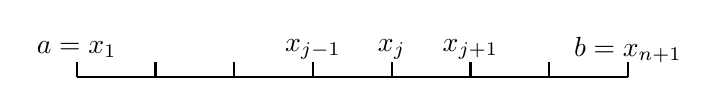
\begin{tikzpicture}
  \draw[color=black, thick] (0,0) -- (1, 0) -- (2, 0) -- (3, 0) -- (4, 0) -- (5, 0) -- (6, 0) -- (7, 0);
  \foreach \x in {0,...,7}
  {
  \draw[color=black, thick] (\x, 0) -- (\x, 0.2);
  }
  \node at (0, 0.35) {$a = x_1$};
    \node at (7, 0.35) {$b = x_{n+1}$};
     \node at (3, 0.35) {$ x_{j-1}$};
      \node at (4, 0.35) {$ x_{j}$};
       \node at (5, 0.35) {$x_{j+1}$};

\end{tikzpicture}
\end{center}



\vspace{1em}

For $X_h^k$, each piece is a polynomial of degree $k$
\vspace{0.5em}


\begin{enumerate}
\item $n(k+1)$ parameters	
\end{enumerate}


\begin{tabular}{c@{\,}r@{\,}l@{\,}c}
  & n(k+1) & parameters  \\
- & (n-1) & match conditions at mesh points to ensure $C^0$  \\
\hline
  & nk+1 &  parameters = dimension of $X^k_h$ 
\end{tabular}
\vspace{0.5em}
For $X^k_{h,0} = X^k_h\cap H^1_0(a,b)$, zero value at 2 boundaries $\Rightarrow$ $nk-1$ parameters.

\vspace{1em}
See $nk+1$ basis functions. Degree of freedom (DOF = $nk+1$). 
\end{frame}


      


%-=-=-=-=-=-=-=-=-=-=-=-=-=-=-=-=-=-=-=-=-=-=-=-=
%	FRAME:
%-=-=-=-=-=-=-=-=-=-=-=-=-=-=-=-=-=-=-=-=-=-=-=-=
\begin{frame}{Construction of linear basis function }
\begin{center}
	    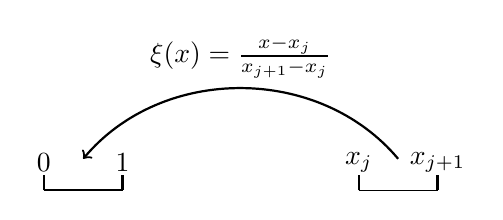
\begin{tikzpicture}
  \draw[color=black, thick] (0,0) -- (1, 0);
  \draw (4,0) -- (5, 0);
  \draw[color=black, thick] (0, 0) -- (0, 0.2);
  \draw[color=black, thick] (1, 0) -- (1, 0.2);
  \draw[color=black, thick] (4, 0) -- (4, 0.2);
  \draw[color=black, thick] (5, 0) -- (5, 0.2);
  
  \draw [color=black, thick, <-]   (0.5, 0.4) to[out=50,in=130]  node[above] {$\xi(x)=\frac{x-x_j}{x_{j+1}-x_j}$} (4.5,0.4);
  
  \node at (0, 0.35) {$0$};
    \node at (1, 0.35) {$1$};
     \node at (4, 0.35) {$ x_{j}$};
      \node at (5, 0.35) {$ x_{j+1}$};

\end{tikzpicture}
\end{center}


The reference element has 2 basis functions called \alert{shape function}.
\begin{columns}[t]
\begin{column}{.5\textwidth}
\begin{center}
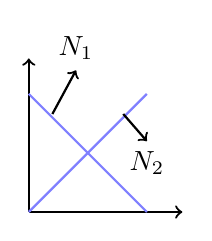
\begin{tikzpicture}[scale=1.5]
  \draw[color=black, thick, ->] (0,0) -- (1.3, 0);
  \draw[color=black, thick, ->](0,0) -- (0, 1.3);
  \draw[color=blue!50,  thick](1,0) -- (0, 1);
  \draw[color=blue!50,  thick](0,0) -- (1, 1);
\draw[->,thick] (0.2, 0.83) -- (0.4,1.2) node [above] {$N_1$};
\draw[->,thick] (0.8, 0.83) -- (1.0,0.6) node [below] {$N_2$};
\end{tikzpicture}
\end{center}
\end{column}

\begin{column}{.5\textwidth}

 Linear functions with cardinal property $N_1(0)=1, N_1(1)=0$ and $N_2(0)=0, N_2(1)=1$
$\Rightarrow N_1(\xi) = 1-\xi, N_2(\xi) = \xi$.



\end{column}

\end{columns}


\end{frame}



%-=-=-=-=-=-=-=-=-=-=-=-=-=-=-=-=-=-=-=-=-=-=-=-=
%	FRAME:
%-=-=-=-=-=-=-=-=-=-=-=-=-=-=-=-=-=-=-=-=-=-=-=-=
\begin{frame}{Global linear basis functions}

Under the map and the shape function, we get 2 basis functions defined on each element $E_j=(x_j,x_{j+1})$: $\phi_j=N_1(\xi(x))$ and $\phi_{j+1}=N_2(\xi(x))$



\begin{center}
	    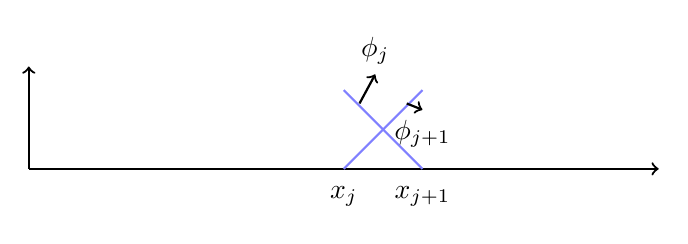
\begin{tikzpicture}
  \draw[color=black, thick] (0,0) -- (1, 0) -- (2, 0) -- (3, 0) -- (4, 0) -- (5, 0) -- (6, 0) -- (7, 0);
\draw[color=black, thick, ->] (0,0) -- (8, 0);
\draw[color=black, thick, ->] (0,0) -- (0, 1.3);
      \node at (4, -0.35) {$ x_{j}$};
       \node at (5, -0.35) {$x_{j+1}$};
  \draw[color=blue!50,  thick](4,0) -- (5, 1);
  \draw[color=blue!50,  thick](5,0) -- (4, 1);
\draw[->,thick] (4.2, 0.83) -- (4.4,1.2) node [above] {$\phi_j$};
\draw[->,thick] (4.8, 0.83) -- (5.0,0.75) node [below] {$\phi_{j+1}$};
\end{tikzpicture}
\end{center}




\begin{center}
	    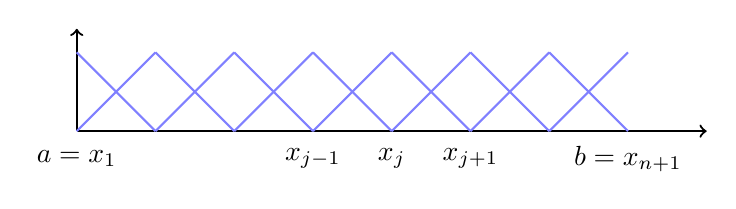
\begin{tikzpicture}
  \draw[color=black, thick] (0,0) -- (1, 0) -- (2, 0) -- (3, 0) -- (4, 0) -- (5, 0) -- (6, 0) -- (7, 0);
  \draw[color=black, thick, ->] (0,0) -- (8, 0);
\draw[color=black, thick, ->] (0,0) -- (0, 1.3);
  \foreach \x in {0,...,6}
  {
  \draw[color=blue!50, thick] (\x, 0) -- (\x+1, 1);
  \draw[color=blue!50, thick] (\x+1, 0) -- (\x, 1);
  }
  \node at (0, -0.35) {$a = x_1$};
    \node at (7, -0.35) {$b = x_{n+1}$};
     \node at (3, -0.35) {$ x_{j-1}$};
      \node at (4, -0.35) {$ x_{j}$};
       \node at (5, -0.35) {$x_{j+1}$};

\end{tikzpicture}
\end{center}

$\Rightarrow (n+1)$ basis fun $\{\phi_j\}\in X^1_h$ (Linear Lagrange element) 
$\Rightarrow \phi_j(x_i) = \delta_{ij}$ and local support, i.e. $\phi_j \neq 0$ only at 
$K_{j-1}\cup K_j$.

\end{frame}



%-=-=-=-=-=-=-=-=-=-=-=-=-=-=-=-=-=-=-=-=-=-=-=-=
%	FRAME:
%-=-=-=-=-=-=-=-=-=-=-=-=-=-=-=-=-=-=-=-=-=-=-=-=
\begin{frame}{Construction of quadratic basis function }

$k=2$, $2n+1$ parameters $\Rightarrow$ $2n+1$ DOFs  $\Rightarrow$ (n+1) mesh points + $n$ extra nodes 
   \begin{center}
  \includegraphics[width=0.8\textwidth]{P2Basis1D.pdf}
     \end{center}
     
  Shape functions on master element: $N_1=(1-\xi)(1-2\xi)$, $N_2=4(1-\xi)\xi$ and $N_3=\xi(2\xi-1)$.  
     
     
       \begin{center}
  \includegraphics[width=0.8\textwidth]{p2.jpg}
     \end{center}
     
\end{frame}





%-=-=-=-=-=-=-=-=-=-=-=-=-=-=-=-=-=-=-=-=-=-=-=-=
%	FRAME:
%-=-=-=-=-=-=-=-=-=-=-=-=-=-=-=-=-=-=-=-=-=-=-=-=
\begin{frame}{Implementation of finite element method}

FEM implementations differ from others in 2 ways:
\begin{enumerate}
\item The stiffness/mass matrices and load vector are computed by doing integrals over each element, called \emph{element stiffness matrices/load vectors}, and assembled into the final global matrices/vectors.
\item Rather than treat Dirichlet boundary conditions using general functions with $u=\phi_0 + \bar{u} \quad (\bar{u} \in V_h^0$). Choose $\phi_0 \in X^k \backslash X_0^k$ so $u\in X^k$ with non zero end basis functions. We do integrals using $u=\sum\limits_{j=1}^{n+1}u_h\phi_j$ then move the corresponding known Dirichlet node values to the right hand side of $A\vec{u}=\vec{b}$.
\end{enumerate}





\end{frame}





%-=-=-=-=-=-=-=-=-=-=-=-=-=-=-=-=-=-=-=-=-=-=-=-=
%	FRAME:
%-=-=-=-=-=-=-=-=-=-=-=-=-=-=-=-=-=-=-=-=-=-=-=-=
\begin{frame}{Implementation of linear finite element method}


For linear Lagrange element,  we have $n$ elements and $n+1$ nodes giving global matrices of size \mbox{$(n+1) \times (n+1)$}. For each element we provide a list of nodes that make up the element in 1D so $K_{\ell}$ has nodes $X_{\ell}$ and $X_{\ell+1}$. The stiffness matrix and load vector are
\begin{align*}
K_{ij}=&\int_a^b D(x) \phi_i' \phi_j' \, dx, \quad \text{for} \quad i,j=1,\dots,\mbox{degrees of freedom}\\
F_i =& \int_a^b f(x)\phi_i(x)\, dx + \mbox{boundary terms}, 
\end{align*}


\end{frame}




%-=-=-=-=-=-=-=-=-=-=-=-=-=-=-=-=-=-=-=-=-=-=-=-=
%	FRAME:
%-=-=-=-=-=-=-=-=-=-=-=-=-=-=-=-=-=-=-=-=-=-=-=-=
\begin{frame}{Observation}


      $K_{ij}=0$ unless $\phi_i'$ and $\phi_j'$ overlap so there are a lot of 0 terms.
Instead we break things over the elements $E_k$:
\begin{align*}
K_{ij} &= \int_a^b D(x) \phi_i' \phi_j' \, dx\\
&= \sum_{\ell=1}^{n} \int_{x_{\ell}}^{x_{{\ell}+1}}D(x) \phi_i' \phi_j' \, dx\\
&= \sum_{\ell=1}^n \int\limits_{E_{\ell}} D(x) \phi_i' \phi_j' \, dx,
\end{align*}
where each individual term in the sum is an element stiffness matrix.
Similarly
\begin{equation*}
F_i = \sum_{\ell=1}^n \int\limits_{E_{\ell}} f(x)\phi_i \, dx.
\end{equation*}


\end{frame}


%-=-=-=-=-=-=-=-=-=-=-=-=-=-=-=-=-=-=-=-=-=-=-=-=
%	FRAME:
%-=-=-=-=-=-=-=-=-=-=-=-=-=-=-=-=-=-=-=-=-=-=-=-=
\begin{frame}{Observation (continue)}


  The only basis functions that are non zero on element $\ell$ are $\phi_{\ell}$ and $\phi_{\ell+1}$. 

\begin{equation*}
F_{E_{\ell}} =
\begin{bmatrix}
\int_{E_{\ell}}f(x)\phi_{\ell} \, dx\\
\int_{E_{\ell}}f(x)\phi_{{\ell}+1} \, dx
\end{bmatrix},
\end{equation*}

\begin{equation*}
K_{E_{\ell}} =
\begin{bmatrix}
\int_{E_{\ell}}D(x)\phi_{\ell}'^2 \, dx & \int_{E_{\ell}}D(x)\phi_{\ell}'\phi_{{\ell}+1}' \, dx \\
\int_{E_{\ell}}D(x)\phi_{{\ell}+1}'\phi_{\ell}' \, dx & \int_{E_{\ell}}D(x)\phi_{{\ell}+1}'^2 \, dx
\end{bmatrix}.
\end{equation*}

\end{frame}


  
      

%-=-=-=-=-=-=-=-=-=-=-=-=-=-=-=-=-=-=-=-=-=-=-=-=
%	FRAME:
%-=-=-=-=-=-=-=-=-=-=-=-=-=-=-=-=-=-=-=-=-=-=-=-=
\begin{frame}{Assemble load vector}
\begin{align*}
\vec{f} &= 
\begin{bmatrix}
( f, \phi_1 )\\
( f, \phi_2 )\\
\vdots\\
\vdots\\
( f, \phi_{n+1} )
\end{bmatrix}
=
\begin{bmatrix}
\int_{x_1}^{x_2} f\phi_1\\
\int_{x_1}^{x_3} f\phi_2\\
\vdots\\
\vdots\\
\int_{x_{n}}^{x_{n+1}} f\phi_{n+1}
\end{bmatrix}
=
\begin{bmatrix}
\int_{x_1}^{x_2} f\phi_1\\
\int_{x_1}^{x_2} f\phi_2\\
0\\
\vdots\\
0
\end{bmatrix}
+
\begin{bmatrix}
0\\
\int_{x_2}^{x_3} f\phi_2 \\
\int_{x_2}^{x_3} f\phi_3 \\
0\\
\vdots
\end{bmatrix}
+ 
\cdots
+
\begin{bmatrix}
0\\
\vdots\\
\vdots\\
\int_{x_n}^{x_{n+1}} f\phi_n\\
\int_{x_n}^{x_{n+1}} f\phi_{n+1}
\end{bmatrix},
\end{align*}



We only need compute element load vector $F_{E_{\ell}}$ and insert it into $(\ell:\ell+1,1)$ locations in $F$.
\end{frame}



%-=-=-=-=-=-=-=-=-=-=-=-=-=-=-=-=-=-=-=-=-=-=-=-=
%	FRAME:
%-=-=-=-=-=-=-=-=-=-=-=-=-=-=-=-=-=-=-=-=-=-=-=-=
\begin{frame}{Assemble stiffness matrix}
\begin{align*}
K &= 
\begin{bmatrix}
K_{E_1} & 0 & \cdots & 0\\
0 & 0 & \cdots & 0\\
\vdots & \vdots & \ddots & 0\\
0 & 0 & \cdots & 0\\
\end{bmatrix}
+ 
\begin{bmatrix}
0 & 0 & \cdots & 0\\
0& K_{E_2}  & \cdots & 0\\
\vdots & \vdots & \ddots & 0\\
0 & 0 & \cdots & 0\\
\end{bmatrix}
+ \cdots +
\begin{bmatrix}
0 & 0 & \cdots & 0\\
0 & 0 & \cdots & 0\\
\vdots & \vdots & \ddots & 0\\
0 & 0 & \cdots & K_{E_n}\\
\end{bmatrix}
\end{align*}

We only need compute element load vector $K_{E_{\ell}}$ and insert it into $(\ell:\ell+1,\ell:\ell+1)$ locations in $K$.
\end{frame}





%-=-=-=-=-=-=-=-=-=-=-=-=-=-=-=-=-=-=-=-=-=-=-=-=
%	FRAME:
%-=-=-=-=-=-=-=-=-=-=-=-=-=-=-=-=-=-=-=-=-=-=-=-=
\begin{frame}{Data structure for implementing linear FEM}



\begin{center}
	    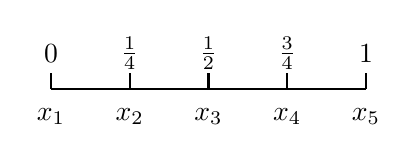
\begin{tikzpicture}
  \draw[color=black, thick] (0,0) -- (1, 0) -- (2, 0) -- (3, 0) -- (4, 0) ;
  \foreach \x in {0,...,4}
  {
  \draw[color=black, thick] (\x, 0) -- (\x, 0.2);
  }
  \node at (0, 0.45) {$ 0$};
    \node at (1, 0.45) {$ \frac{1}{4}$};
     \node at (2, 0.45) {$ \frac{1}{2}$};
      \node at (3, 0.45) {$ \frac{3}{4}$};
       \node at (4, 0.45) {$1$};
\node at (0, -0.35) {$ x_1$};
    \node at (1, -0.35) {$ x_{2}$};
     \node at (2, -0.35) {$ x_{3}$};
      \node at (3, -0.35) {$ x_{4}$};
       \node at (4, -0.35) {$x_{5}$};


\end{tikzpicture}
\end{center}


\begin{equation*}
\text{node} = \begin{bmatrix}
	x_1\\
	x_2\\
	x_3\\
	x_4\\
	x_5
\end{bmatrix}
=
\begin{bmatrix}
	0\\
	\frac{1}{4}\\
	\frac{1}{2}\\
	\frac{3}{4}\\
	1
	\end{bmatrix}
	\quad \quad
	\text{elem} = \begin{bmatrix}
	1 & 2 \\
	2 & 3\\
	3 & 4\\
	4 & 5\\
\end{bmatrix}
\end{equation*}


elem is just the local numbering of local points to the global numbering of global points

\end{frame}





%-=-=-=-=-=-=-=-=-=-=-=-=-=-=-=-=-=-=-=-=-=-=-=-=
%	FRAME:
%-=-=-=-=-=-=-=-=-=-=-=-=-=-=-=-=-=-=-=-=-=-=-=-=
\begin{frame}{Pseudo code}

A = sparse(n+1, n+1);


b = zeros(n+1,1);


for j = 1:n



$\quad\quad x_j = node(elem(j,1));$



$\quad\quad x_{j+1} = node(elem(j,2));$



$\quad\quad K_{E_j} = elem\_stiff(x_j, x_{j+1}, D); $ \% compute element stiffness matrix



$\quad\quad F_{E_j} = elem\_load(x_j, x_{j+1}, f); $ \% compute element load vector



$\quad\quad A(elem(j,:), elem(j,:)) = A(elem(j,:), elem(j,:)) + K_{E_j}; $ 



$\quad\quad b(elem(j,:), 1) = b(elem(j,:), 1) + F_{E_j}; $ 



end





You should write funs to compute element matrices/vectors which can be done by mapping into master element. 

\end{frame}






%-=-=-=-=-=-=-=-=-=-=-=-=-=-=-=-=-=-=-=-=-=-=-=-=
%	FRAME:
%-=-=-=-=-=-=-=-=-=-=-=-=-=-=-=-=-=-=-=-=-=-=-=-=
\begin{frame}{Computation of elementary matrices/vector}
Map each integral to the master element and then integrate over $[0,1]$.
\begin{align*}
\int_{x_j}^{x_{j+1}}f(x)\phi_{j} \, dx=h_j \int_0^1 f(x(\xi))N_1(\xi) \,d\xi, \\
\int_{x_j}^{x_{j+1}}f(x)\phi_{j+1} \, dx=h_j \int_0^1 f(x(\xi))N_2(\xi) \,d\xi.
\end{align*}


Similarly, 
\begin{align*}
&\int_{x_j}^{x_{j+1}}\frac{d\phi_{j}(x)}{dx}\frac{d\phi_{j+1}(x)}{dx} \, dx=
\int_{0}^{1}\frac{d\phi_{j}(x(\xi))}{dx}\frac{d\phi_{j+1}(x(\xi))}{dx} \frac{dx}{d\xi}\, d\xi\\
=&\int_{0}^{1}\frac{dN_1(\xi)}{d\xi}\frac{d\xi}{dx}\frac{dN_2(\xi)}{d\xi}\frac{d\xi}{dx} \frac{dx}{d\xi}\,d\xi
= \int_{0}^{1}\frac{dN_1(\xi)}{d\xi}\frac{1}{h_j}\frac{dN_2(\xi)}{d\xi}\frac{1}{h_j} h_j\,d\xi\\
=& \frac{1}{h_j}\int_{0}^{1}\frac{dN_1(\xi)}{d\xi}\frac{dN_2(\xi)}{d\xi}\,d\xi.
\end{align*}


\end{frame}



%-=-=-=-=-=-=-=-=-=-=-=-=-=-=-=-=-=-=-=-=-=-=-=-=
%	FRAME:
%-=-=-=-=-=-=-=-=-=-=-=-=-=-=-=-=-=-=-=-=-=-=-=-=
\begin{frame}{Elementary matrices/vector of quadratic element}
\begin{equation*}
F_{E_1}=
\begin{bmatrix}
( f,\phi_1 )\\
( f,\phi_2 )\\
( f,\phi_3 )
\end{bmatrix},
\quad 
F_{E_2}=
\begin{bmatrix}
( f,\phi_3 )\\
( f,\phi_4 )\\
( f,\phi_5 )
\end{bmatrix},
\end{equation*}


\begin{equation*}
K_{E_1}=
\begin{bmatrix}
K_{11} & K_{12} & K_{13}\\
K_{21} & K_{22} & K_{23}\\
K_{31} & K_{32} & K_{33}
\end{bmatrix},
\quad 
K_{E_2}=
\begin{bmatrix}
K_{33} & K_{34} & K_{35}\\
K_{43} & K_{44} & K_{45}\\
K_{53} & K_{54} & K_{55}
\end{bmatrix},
\end{equation*}

\end{frame}




%-=-=-=-=-=-=-=-=-=-=-=-=-=-=-=-=-=-=-=-=-=-=-=-=
%	FRAME:
%-=-=-=-=-=-=-=-=-=-=-=-=-=-=-=-=-=-=-=-=-=-=-=-=
\begin{frame}{Data structure for implementing quadratic FEM}



\begin{center}
	    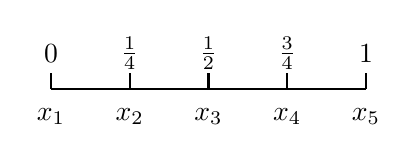
\begin{tikzpicture}
  \draw[color=black, thick] (0,0) -- (1, 0) -- (2, 0) -- (3, 0) -- (4, 0) ;
  \foreach \x in {0,...,4}
  {
  \draw[color=black, thick] (\x, 0) -- (\x, 0.2);
  }
  \node at (0, 0.45) {$ 0$};
    \node at (1, 0.45) {$ \frac{1}{4}$};
     \node at (2, 0.45) {$ \frac{1}{2}$};
      \node at (3, 0.45) {$ \frac{3}{4}$};
       \node at (4, 0.45) {$1$};
\node at (0, -0.35) {$ x_1$};
    \node at (1, -0.35) {$ x_{2}$};
     \node at (2, -0.35) {$ x_{3}$};
      \node at (3, -0.35) {$ x_{4}$};
       \node at (4, -0.35) {$x_{5}$};


\end{tikzpicture}
\end{center}


\begin{equation*}
\text{node} = \begin{bmatrix}
	x_1\\
	x_2\\
	x_3\\
	x_4\\
	x_5
\end{bmatrix}
=
\begin{bmatrix}
	0\\
	\frac{1}{4}\\
	\frac{1}{2}\\
	\frac{3}{4}\\
	1
	\end{bmatrix}
	\quad \quad
	\text{elem} = \begin{bmatrix}
	1 & 2 \\
	2 & 3\\
	3 & 4\\
	4 & 5\\
\end{bmatrix}
\quad \quad
	\text{elem2dof} = \begin{bmatrix}
	1 & 6 &2 \\
	2 & 7 & 3\\
	3 & 8& 4\\
	4 & 9& 5\\
\end{bmatrix}
\end{equation*}


elem2dof is just the  numbering of local basis functions to the global numbering of global basis functions

\end{frame}



%-=-=-=-=-=-=-=-=-=-=-=-=-=-=-=-=-=-=-=-=-=-=-=-=
%	FRAME:
%-=-=-=-=-=-=-=-=-=-=-=-=-=-=-=-=-=-=-=-=-=-=-=-=
\begin{frame}{Pseudo code of quadratic element}

A = sparse(n+1, n+1);


b = zeros(n+1,1);


for j = 1:n



$\quad\quad x_j = node(elem(j,1));$



$\quad\quad x_{j+1} = node(elem(j,2));$



$\quad\quad K_{E_j} = elem\_stiffp2(x_j, x_{j+1}, D); $ \%element stiffness matrix



$\quad\quad F_{E_j} = elem\_loadp2(x_j, x_{j+1}, f); $ \% compute element load vector



$\quad\quad A(elem2dof(j,:), elem2dof(j,:)) = A(elem2dof(j,:), elem2dof(j,:)) + K_{E_j}; $ 



$\quad\quad b(elem2dof(j,:), 1) = A(elem2dof(j,:), 1) + F_{E_j}; $ 



end





You should write funs to compute element matrices/vectors which can be done by mapping into master element. 

\end{frame}

%-=-=-=-=-=-=-=-=-=-=-=-=-=-=-=-=-=-=-=-=-=-=-=-=
%	FRAME:
%-=-=-=-=-=-=-=-=-=-=-=-=-=-=-=-=-=-=-=-=-=-=-=-=
\begin{frame}{Galerkin orthogonality}

The \alert{bilinear form} (or inner product) defined by the ODE
\begin{equation*}
a(u,v)= \int_a^b D(x) u' v' + q(x) u v \  dx,
\end{equation*}
which also induced an norm called \alert{energy norm} 
$$\|v\|_E^2=\int_a^b D(x) |v'|^2 + q(x) v^2\,dx.$$


\alert{Galerkin orthogonality}:
\begin{equation*}
a(u-u_h,v_h)=0  \ \ \   \forall v_h \in V_h,
\end{equation*}




\end{frame}



%-=-=-=-=-=-=-=-=-=-=-=-=-=-=-=-=-=-=-=-=-=-=-=-=
%	FRAME:
%-=-=-=-=-=-=-=-=-=-=-=-=-=-=-=-=-=-=-=-=-=-=-=-=
\begin{frame}{Properties of bilinear form}

Two properties:
\begin{itemize}
	\item Coercivity: $c \|u\|_{H^1(a,b)}^2 \le a(u, u)$ (Poincar\'e's Lemma).
	\item Continuity: $a(u, v) \le C\|u\|_{H^1(a,b)}\|v\|_{H^1(a,b)} $ (Cauchy-Schwartz Inequality)
\end{itemize}

\begin{lem}[(Lax-Miligram)]
	f Let $a(\cdot, \cdot)$ be a bounded coercive and continuous bilinear form on a Hilbert space $H^1_0(a,b)$. Then for any function $f\in L^2(a,b)$,  there exists a unique $u$ in $H^1_0(a,b)$ such that
	\begin{equation*}
		a(u,v) = (f, v), \quad v\in H^1_0(a, b). 
	\end{equation*}
\end{lem}


 \alert{Sufficient condition} for this weak formulation to have a unique solution.

\end{frame}





%-=-=-=-=-=-=-=-=-=-=-=-=-=-=-=-=-=-=-=-=-=-=-=-=
%	FRAME:
%-=-=-=-=-=-=-=-=-=-=-=-=-=-=-=-=-=-=-=-=-=-=-=-=
\begin{frame}{Ce\`a's Lemma}

\begin{lem}
	a Let $u_h$ be the finite element solution of the model problem. Assume $V_h$ is a subspace of $H^1$, then we have 
	\begin{equation*}
\|u-u_h\|_E =  \min\limits_{w_h\in V_h} \|u-w_{h}\|_E,
\end{equation*}
\end{lem}



\alert{Best approximation property}:  the Galerkin solution is the best approximation to $u$ from all the functions in $V_h$.

\end{frame}




%-=-=-=-=-=-=-=-=-=-=-=-=-=-=-=-=-=-=-=-=-=-=-=-=
%	FRAME:
%-=-=-=-=-=-=-=-=-=-=-=-=-=-=-=-=-=-=-=-=-=-=-=-=
\begin{frame}{Error estimate}

\begin{thm}
a Assume $u \in H^s$ for $s \ge 2$ and $u_h \in V_h=X_h^k$. Then:
\begin{equation*}
\|u-u_h\|_{H_0^1} \le C h^l \|u\|_{H^{l+1}},
\end{equation*}
where $l=\min\{k,s-1\}$.

Also,
\begin{equation*}
\|u-u_h\|_{L^2} \le C h^{l+1}\|u\|_{H^{l+1}}.
\end{equation*}
\end{thm}



Assume $u$ is smooth enough. $k$th order in $H^1$ norm and $(k+1)$th order in $L^2$ norm. 

\end{frame}



%-=-=-=-=-=-=-=-=-=-=-=-=-=-=-=-=-=-=-=-=-=-=-=-=
%	FRAME:
%-=-=-=-=-=-=-=-=-=-=-=-=-=-=-=-=-=-=-=-=-=-=-=-=
\begin{frame}[standout]
  End of week 3!
\end{frame}

\appendix



\end{document}
